% !Mode:: "TeX:UTF-8"
% !TEX root = ..\thesis.tex
\chapter{装配生产线分析及模型建立}
本章将对装配线生产进行分析,指出现有计划安排和调度存在的主要问题,然后针对这些问题,提出合理解决方案,并对其进行分析和数学建模。


\section{生产线分析}
课题研究对象是该汽车电子公司的总装生产线,是典型的流水车间,每条流水线负责同一主机厂的不同品种产品总装流程。装配生产根据订单批量进行安排,根据先到先服务(FCFS)规则生成任务队列。

生产线分析包括上述这些差别及其产生的影响或效果,具体描述从订单、装配到交付的流程,并分析现行调度方案的一些指标。

\subsection{现行流程描述}
现行下达订单到交付的流程如\reff{fig:orderflow}所示,销售人员接到客户订单,在确认工期后,将之送达计划部门,制定主生产计划(MRP),随后根据产品特性安排采购与厂内加工。根据任务队列与批量进行产品总装,通过质检包装后,销售人员安排运输送达至客户。
订单到达会立即安排入其对应的主机厂专用产线,当同一主机厂有多个订单同时到达时,则根据最早交货期(EDD)规则进行生产调度。

本课题的研究对象是流程中的总装调度安排,
\subsection{现行调度方案}
任务下达到车间时,需要根据订单队列及其批量进行调度安排,


现行调度方案逻辑简单,执行力强,每条装配线可分时生产不同品种的产品,而且按照厂家来安排组织生产,方便了管理。


\subsection{主要问题}
现行调度方案存在诸多问题,例如多条装配线负荷不均衡,有的任务过重,有的任务不足,负荷不均衡,一条装配线上装配的产品工艺相似性较低,导致换线时间增加,产生更长的等待。

根据现行调度情况进行问题分析,可以归纳其主要存在问题如下:
\renewcommand{\labelenumi}{(\theenumi)}
\begin{asparaenum}
\item 产线利用率低
\suspend{asparaenum}

产线利用率低主要体现在存在大量换线时间,一方面由于产线等待队列由FCFS 规则产生,同时到达的订单也只是根据EDD 规则安排,没有考虑品种装配流程间的相似性。当这种差异很大时,必然会增加换线时间,进而增加了任务间的等待。另一方面,由于产线的专用性,当有多条产线都能处理某个任务时,该任务只能在订单来自的主机厂专线上生产,闲置了可用线的生产能力。
\resume{asparaenum}
\item 生产不均衡
\suspend{asparaenum}

这里的生产均衡和混流生产中的均衡生产稍有差别,此处的不均衡现象更为宏观。来自不同主机厂的任务在不同产线上进行处理,这样一来,订单较多、较频繁的主机厂产线总是会处于繁忙状态,而订单较少的产线则呈现为停线等待居多。这种不均衡现象直接导致产能的巨大浪费,同时也间接导致了换线时间增加,因为不均衡的生产业表面订单较为集中。突破专线限制可以解决宏观不均衡问题,虽然细分到单条线上的混流生产可以近一步均衡化生产,但其需要较高的管理投入,可以考虑折衷。
\resume{asparaenum}
\item 工艺及设备和生产需求不匹配
\suspend{asparaenum}

各流水线需要有多品种加工的能力,故线上需要有相应加工工艺的设备,而时常不同主机厂所需产品可能有很高的相似性,这使得同样的设备需要在多条流水线上设置,尤其对于加工时间较短、处理批量较少的作业,过多的设备徒增成本与闲置。另一方面,加工时间厂、处理批量大的作业,台少的设备不利于生产效率,导致在制品增爹。
\resume{asparaenum}
\item 工期可控性低
\suspend{asparaenum}

工期的可控性低主要体现在应变插单的问题上,现行调度采用的是不可中断的流水作业,各流水线只能按其队列顺序进行装配作业,由于这样安排没有顾及工期的先后即订单的具体情况,导致大部分订单都需要延期交货,也存在较多订单的过早完工,增加了库存。此外,虽然插单可以较为合理安排订单加工顺序,而然会到来额外的切换时间,需要权衡考虑。
\resume{asparaenum}
\item 产线冗余度高
\end{asparaenum}

前面几大问题已经涉及到了一些浪费现象,除了这些之外,该厂制造二部共有8个装配车间,每个装配车间有7--8条总装流水线,然而由于流水线是按主机厂进行分配,存在较高的冗余度,前面提到的产线间设备类似属于其中之一。产线的冗余还包括作业及管理人员,辅助设置,场地空间,相关能源等。

上述问题为研究对象的目前的主要问题,并对其产生原因进行分析,这为改进调度方案明确了方向。具体改进过程需要通过建模分析。

\section{模型建立}
为制定合理调度方案,改善装配流水线现状,首先需要确定改进目标,进而根据目标的可行性,建立数学模型。
因此,本节将结合实际情况,权衡投入和效益,建立适合本课题研究对象的混线装配生产模型。
\subsection{目标改进及...}
目前的生产现状主要是存在各主机厂的专用流水线,所以首要的改进是突破专用线的生产界限。如此一来,生产线可以加工多家主机厂的订单,形成所谓的混线生产,是较混流生产为宏观的均衡化生产,如\reff{fig:orderschedule}所示\footnote{\reff{fig:orderschedule}中订单a -- b 表示主机厂a 的第b 个订单}
。其次,适当允许任务中断,安排插单作业,可以近一步改善现有浪费,而且增加生产应变能力。
\begin{figure}[h]
\centering
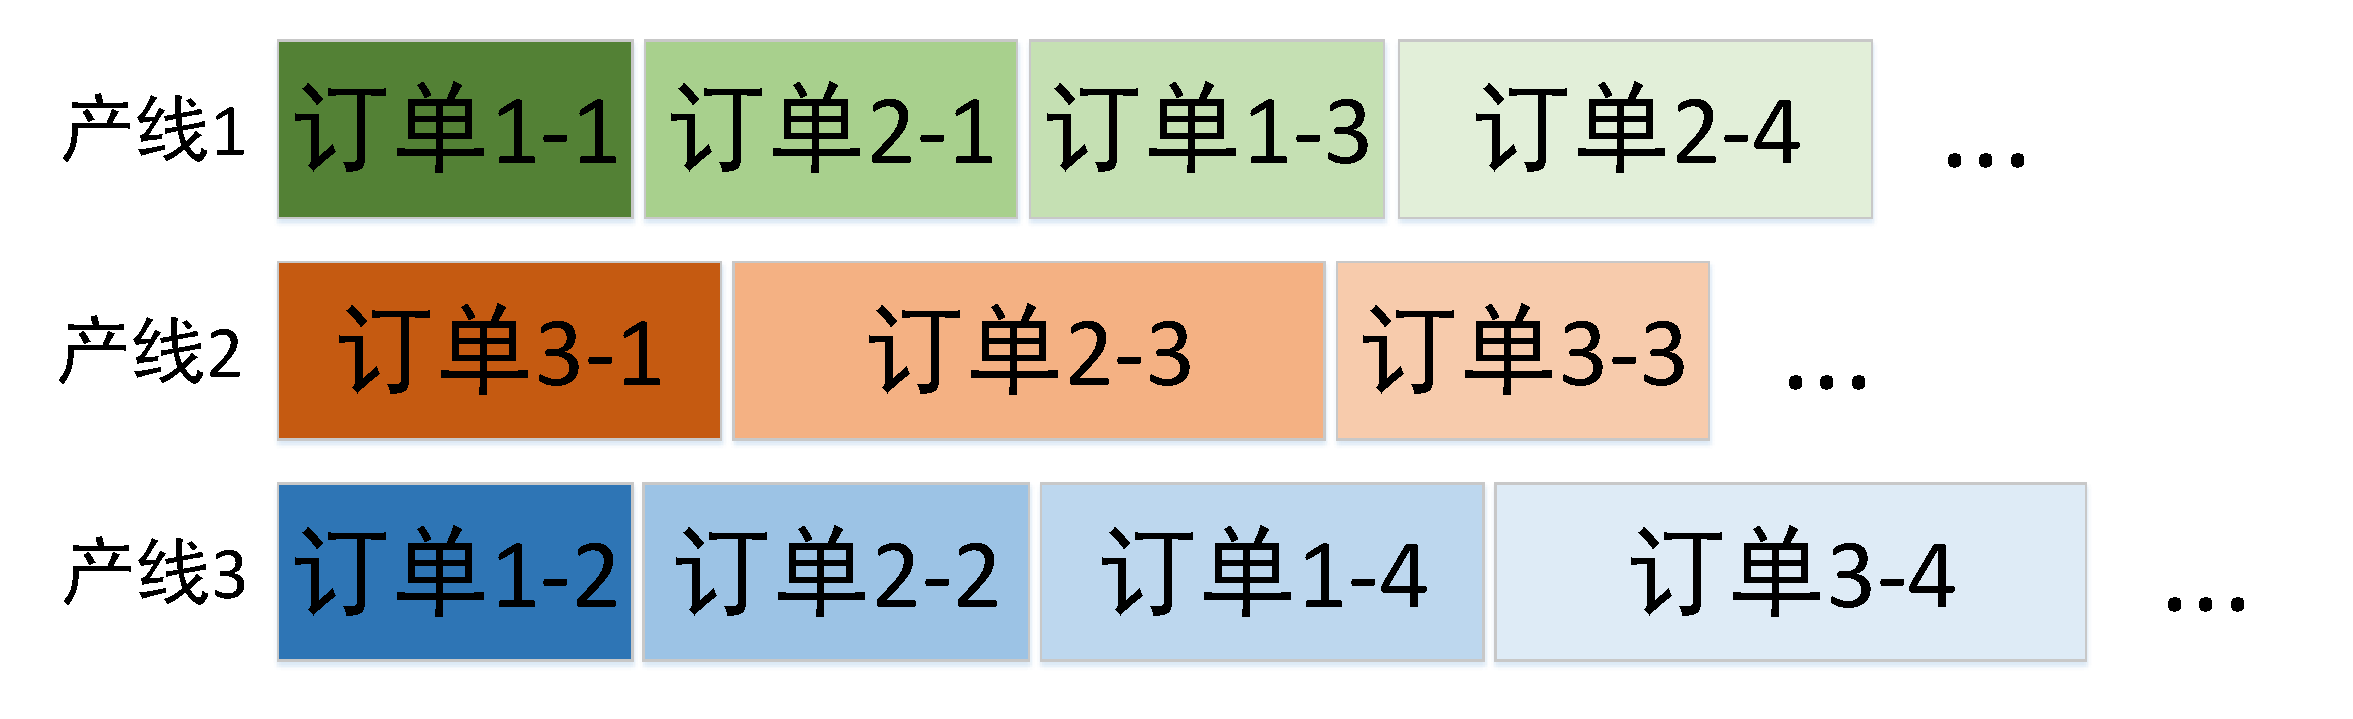
\includegraphics[width = 8cm]{oredrschedule.pdf}
\caption{3条产线的混线装配生产示意\label{fig:orderschedule}}
\end{figure}

根据这样的目标,对所需生产的订单进行排列组合,较为均匀地安排在各流水线上,以期获得均衡的生产线利用率、减少换线时间浪费、缩短完工时间、降低生产成本。此外,虽然实施完全均衡化生产需要有较高的管理水平和投入,但是适当的混流(即考虑投入产出关系后)可以有效提高产线性能,需要确定混流程度。

....将不同产品的订单看作为作业,流水线上的各装配工位或机器看作处理单元,那么流水线上的作业流程可以看作是各作业按固定顺序经过线上的处理单元进行处理。

\subsection{符号说明}
为了方便问题描述,符号说明如下:

\begin{center}
\begin{supertabular}{ll}
$n$ & 订单数量\\
$m$ & 流水线数量\\
$j$ & 订单标记,$j = 1,2,...,n$\\
$l$ & 流水线标记,$l = 1,2,...,m$\\
$n_j$ & 订单$j$的作业(需求)量\\
$m_j$ & 订单$j$所需处理单元数量\\
$j_i$ & 订单$j$的处理单元标记,其中$i = 1,2,...,m_j$\\
$(i,j)$ & 表示作业$j$在流水线$i$上装配\\
$p_{i,j}$ & 订单$j$中单个作业在处理单元$j_i$上的处理时间\\
$d_j$ & 订单$j$的交货期\\
$r_j$ & 订单$j$进入流水线系统日期,是其最早可开始时间\\
$C_j$ & 订单$j$的完成时间\\
$C_{\max}$ & 制造期\\

%%%%%%%%%%%%
$r$ & 批次中的位置标记\\
$b$ & 工段中的批数,$b\geqslant2$\\
$c$ & 工段1的批量\\
$J$ & 需要调度的作业集合,$J=\{1,2,...,n\}$\\
$p_{aj}$ & $J_j$在工段$a$的单件处理时间,$p_{aj}=p_a$\\
$p_{1j}$ & $J_j$在工段1的处理时间,$p_{1j}=p_1$\\
$p_{2j}$ & $J_j$在工段1的处理时间\\
$s_a$ & 在工段1的作业换线时间\\
$s_b$ & 在工段2的批次换线时间\\
$s_{f1}$ & 在工段1的产品簇换线时间\\
$s_{f2}$ & 在工段2的产品簇换线时间\\
$f_j$ & $J_j$的产品簇,$f_j=1,2,3,4$\\
$f_{1,[i,r]}$ & 在工段1中安排在第$r$批次作业$[i,r]$的产品簇 \\
$f_{2,[j]}$ & 在工段2中安排在第$j$批次$J_{[j]}$的产品簇 \\
$k_{1,[i,r]}$ & \begin{numcases}{=}
{\liuhao 0 }&{\liuhao 在工段1,如果作业$[i,r]$和它的前继作业同属一个产品簇}\notag\\
{\liuhao 1 }&{\liuhao 其他情况} \notag
\end{numcases}\\[5pt]
$k_{2,[j]}$ & \begin{numcases}{=}
{\liuhao 0 }&{\liuhao 在工段2,如果$J_[j]$和它的前继作业同属一个产品簇}\notag\\
{\liuhao 1 }&{\liuhao 其他情况} \notag
\end{numcases}\\
$S$ & 已调度的作业集合\\
$S_U$ & 未调度作业集合\\
$B$ & 已调度批集合\\
$B_i$ & 工段1的第$i$批,$B_i\subset B$\\
$p_1(B_i)$ & 工段1的$B_i$处理时间\\
$D_j$ & $J_j$的交货期\\
$d_j$ & $J_j$的工期\\
$d_{[j]}$ & $J_{[j]}$在工段2的工期\\
$C_{1,[i]}$ & 批$i$在工段1的完工时间\\
$C_{2,[j]}$ & $J_{[j]}$在工段2的完工时间\\
$T_j$ & $J_{[j]}$的滞后时间\\
\end{supertabular}
\end{center}
%%%%%%%%%%%%%%%%%%%%%%%%%%

\subsection{相关假设}

假设流水线、作业和处理单元数量有限,
不同流水线上加工同一品种作业的处理时间相同,
本课题的调度研究不涉及具体的装配工艺流程,故假定不同产品的工艺区别只能体现在处理时间和设备准备时间,
按队列生产时,需要考虑切换准备时间,作业准备时间只和其前继作业有关,并且准备时间事先已知。

考虑插单时,正在处理的作业可以被中断,一旦作业中断,该作业中正在处理的产品需要继续完成,未开始处理的产品则进入中断队列。被中断作业在后面继续完成剩下部分时,可以选择任意流水线,仍然要考虑产线准备时间

\subsection{目标函数}
本课题期望通过合理调度,达到提高产线利用率、减少浪费、缩短制造期、提高应变能力、减少库存、降低生产成本等目标,这些目标有着内在联系,所以在设计目标函数的时候,不必把每样都列入其中。
需要定义订单的延时函数:

\begin{numcases}{L_j=}
C_j - d_j & if $C_j > d_j$ \notag\\
0 & otherwise \notag
\end{numcases}

适时适量生产,最小化加权延时和完成时间,即:
\begin{gather}
\min\  z = \sum_{j=1}^nw'_j(C_j - r_j) + \sum_{j=1}^nw''_jL_j
\end{gather}
\subsection{约束条件}


\section{小结}